\clearpage
\section{Aprendizado Não Supervisionado}

Na aprendizagem não supervisionada, os dados de entrada não possuem classes (ou rótulos) e o objetivo do algoritmo é descrever estruturas dentro do conjunto de dados. Uma vez que os dados não são classificados, não existe um erro ou uma recompensa, o que distingue o aprendizado não supervisionado da aprendizagem supervisionada ou por esforço. A aprendizagem não supervisionada é bastante utilizada para resumir e explicar as principais características dos dados \cite{jordan2004}.


\subsection{Clusterização}
\label{sec:clusterização}

Quando temos um conjunto grande de elementos, naturalmente tentamos estabelecer padrões entre eles. Uma forma natural de definir padrões em um conjunto é analisar a distância entre seus componentes. Dessa forma, quanto mais parecidos dois elementos são, mais próximos eles estão. A figura abaixo mostra um conjunto de elementos com duas características: forma (quadrado, círculo e triângulo) e cor (tons de vermelho, verde e azul). Ao lado temos os mesmos elementos agrupados em três conjuntos com características semelhantes. No grupo 1, por exemplo, todos os elementos possuem uma tonalidade de vermelho e o formato quadrado.

\begin{figure}[h]
  \centering
  \begin{subfigure}{.5\textwidth}
    \centering
    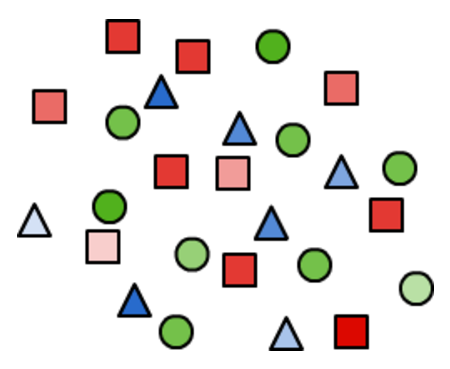
\includegraphics[scale=0.8]{figuras/ungroup-elements.eps}
    \label{fig:ungroup-elements}
    \caption{Elementos não agrupados}
  \end{subfigure}%
  \begin{subfigure}{.5\textwidth}
    \centering
    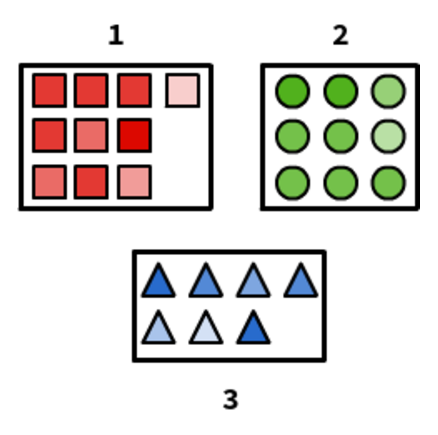
\includegraphics[scale=0.8]{figuras/group-elements.eps}
    \label{fig:group-elements}
    \caption{Elementos agrupados}
  \end{subfigure}
  \caption{Exemplo de clusterização}
\end{figure}

A clusterização é uma técnica da mineração de dados que consiste, justamente, em realizar o procedimento descrito acima: organizar um conjunto de elementos, usualmente representados por vetores ou pontos em um espaço multidimensional, em \textit{clusters} (ou agrupamentos), de acordo com alguma medida de similaridade. Ela representa uma das principais etapas da análise de dados, denominada análise de \textit{clusters} \cite{jain1999}.

Não existe uma técnica de clusterização universal capaz de revelar toda a variedade de estruturas que podem estar presentes em conjuntos de dados multidimensionais. Diferentes algoritmos dependem implicitamente de certas hipóteses a respeito da forma dos clusters, da definição da medida de similaridade e dos critérios de agrupamento \cite{estivill2002}.

\subsubsection{Algoritmo \textit{k-means}}
\label{sub:k_means}

O algoritmo de clusterização \textit{k-means}, proposto por \citeonline{lloyd1957}, tem o objetivo de dividir \(N\) elementos em \(k\) grupos, onde cada elemento pertence ao \textit{cluster} mais próximo. O valor de \(k\) deve ser informado a priori, sendo menor que a quantidade de elementos.

Os passos do algoritmo são:

\begin{enumerate}
  \item \textbf{Gerar centroides:} neste passo os \(k\) centroides recebem valores iniciais. O valor inicial dos centroides podem ser definidos randomicamente, através de uma Gaussiana (com média e variância estimados a partir do conjunto de elementos) ou escolhendo aleatoriamente \(k\) dos \(N\) elementos como centroides iniciais ou definindo-os como centroides de \(k\) grupos escolhidos aleatoriamente a partir dos dados iniciais.
  \begin{figure}[h]
    \centering
    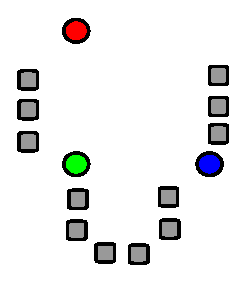
\includegraphics[scale=0.6]{figuras/kmeans-1.eps}
    \caption{k centroides (coloridos) recebem valores iniciais.}
  \end{figure}
  \item \textbf{Calcular distâncias:} aqui são calculadas as distâncias entre cada ponto e cada centroide. É a parte com maior peso computacional do algoritmo, já que o calculo é realizado para cada ponto.
  \item \textbf{Classificar os pontos:} cada ponto deve ser classificado de acordo com a distância entre ele e o centroide de cada \textit{cluster}. O ponto pertencerá ao \textit{cluster} cujo centroide está mais próximo. O algoritmo converge quando, em uma iteração, nenhum ponto mudar de \textit{cluster}.
  \begin{figure}[h]
    \centering
    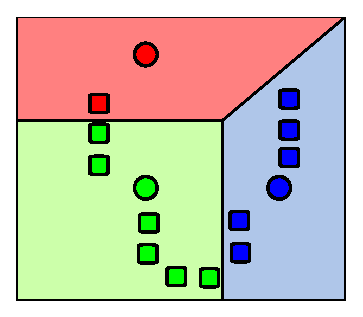
\includegraphics[scale=0.6]{figuras/kmeans-2.eps}
    \caption{Cálculo das distâncias entre os pontos e os centroides.}
  \end{figure}
  \item \textbf{Calcular novos centroides:} para cada \textit{cluster}, um novo centroide é definido como a média de todos os pontos.
  \begin{figure}[h]
    \centering
    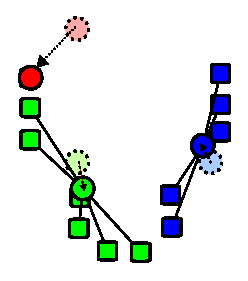
\includegraphics[scale=0.6]{figuras/kmeans-3.eps}
    \caption{Novos centroides definidos pela media dos elementos do \textit{cluster}.}
  \end{figure}
  \item \textbf{Repetir até convergir:} retorna ao passo 2. Como o resultado do algoritmo depende da escolha dos centroides iniciais, a convergência não é garantida ou ele converge para uma solução sub-ótima. Por isso, normalmente o algoritmo é executado várias vezes.
  \begin{figure}[h]
    \centering
    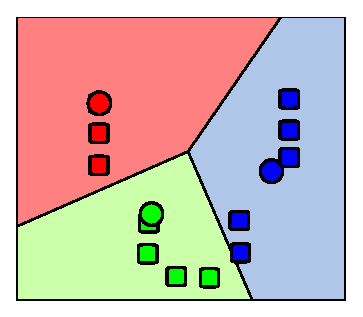
\includegraphics[scale=0.6]{figuras/kmeans-4.eps}
    \caption{O algoritmo converge quando nenhum ponto muda de \textit{cluster}.}
  \end{figure}
\end{enumerate}

Mudanças de escala ou de unidade de medidas para determinadas coordenadas dos elementos podem afetar a análise \cite{cole1998}. Sugere-se, então, que seja feito o processo de normalização (\textit{whitening}) dos dados antes da clusterização. A normalização consiste em ajustar a escala das distâncias de forma que os valores fiquem em intervalos padronizados, normalmente com média nula e variância 1.


\subsubsection{\textit{Latent Dirichlet Allocation - LDA}}

O \textit{LDA} foi proposto por \citeonline{pritchard} em uma aplicação inicial na biologia. Em seu modelo, \citeonline{pritchard} utilizam dados de genótipos multi locus para inferir estruturas populacionais e associar cada indivíduos a uma mistura de populações parentais. Dessa forma, também conseguem estudar zonas híbridas entre as populações e identificar indivíduos migrantes e misturados. A aplicação desse modelo no processamento de linguagem natural foi proposta independentemente por \citeonline{blei}, onde os documentos são tratados como os indivíduos e as populações passam a ser tópicos.

No contexto do processamento de linguagem natural, um documento, ou palavra, pode ser representado por uma mistura de vários tópicos, o que permite uma melhor desambiguação dos termos e uma definição de tópicos mais precisa \cite{girolami}. Usamos como exemplo as seguintes frases:

\begin{enumerate}
  \item Eu \textbf{como peixe}.
  \item \textit{Peixes} são \textit{animais}.
  \item Meu \textit{gato} \textbf{come peixe}.
\end{enumerate}

O \textit{LDA} poderia classificar os termos em \textbf{negrito} como pertencentes ao \textbf{Tópico C}, que poderia ser rotulado como ``\textbf{comida}''. Da mesma forma, as palavras em \textit{itálico} também poderiam ser agrupadas em um \textit{Tópico A}, rotulado como ``\textit{animais}''.

Esse modelo tenta inferir duas tabelas de probabilidade: estrutura (\(P\)) e mistura (\(Q\)). Em \(P\) temos as probabilidades de um termo estar presente em uma frase de cada tópico, sendo que essas probabilidades são independentes entre si. Já em \(Q\), temos as probabilidades de cada documento pertencer à cada tópico, mas, nesse caso, as probabilidades devem somar um total de 100\%. Foram utilizados dados hipotéticos nas tabelas abaixo apenas para ajudar na explicação.

\begin{table}[h]
\centering
\begin{tabular}{|c|c|c|}
\hline
\textbf{Termo/Tópico} & \textbf{Comida} & \textbf{Animal} \\ \hline
comer & 0.9 & 0.3 \\ \hline
peixe & 0.5 & 0.6 \\ \hline
animal & 0.2 & 0.8 \\ \hline
gato & 0.2 & 0.8 \\ \hline
\end{tabular}
\caption{Tabela de Estrutura dos Termos (P)}
\label{tabelap}
\end{table}

\begin{table}[h]
\centering
\begin{tabular}{|c|c|c|}
\hline
\textbf{Documento/Tópico} & \textbf{Comida} & \textbf{Animal} \\ \hline
Frase 1 & 0.8 & 0.2 \\ \hline
Frase 2 & 0.1 & 0.9 \\ \hline
Frase 3 & 0.6 & 0.4 \\ \hline
\end{tabular}
\caption{Tabela de Mistura dos Documentos (Q)}
\label{tabelaq}
\end{table}

Essas tabelas influenciam diretamente uma à outra, ou seja, se um termo começa a ser predominante em determinado tópico, o documento a qual ele pertence passa a tender à esse tópico. Da mesma forma que se um documento começar a tender a um tópico, seus termos também serão favorecidos neste tópico.

Para se obter o conteúdo de cada tópico, basta observar as colunas de \(P\), onde teremos uma \textit{bag of words} contendo a probabilidade de todos os termos pertencerem à esse tópico. Analisando as linhas de \(Q\), temos as misturas de tópicos de cada documento. Vale notar que, por ser uma mistura de tópicos, o \textit{LDA} dificilmente vai atribuir um documento à um único tópico com 100\% de pertencimento.

Para chegar à essa conclusão, o \textit{LDA} segue três passos:

\begin{itemize}
  \item \textbf{Quantidade de tópicos:} assim como no \textit{k-means}, o primeiro passo é definir a quantidade de tópicos que serão obtidos ao final da análise. Esse número pode ser obtido através de uma análise prévia dos dados ou simplesmente por uma escolha aleatória.
  \item \textbf{Inicializar as tabelas \(P\) e \(Q\):} É definida uma distribuição de tópico inicial para cada documento, que será atualizado no passo seguinte. A escolha desses tópicos se dá de forma semi-aleatória, de acordo com a distribuição de \textit{Dirichlet}, ou seja, valores aleatórios entre 0 e 1 com a restrição de que a soma deles deve ser 1. As probabilidades \(P\) podem ser definidas de forma uniforme para todos os termos: \(P=0.5\).
  \item \textbf{Analisar e atualizar os tópicos:} Para cada palavra, em todos os documentos, a definição do tópico é atualizada de acordo com dois critérios: o quanto essa palavra é predominante  entre os tópicos e quão predominante são os tópicos entre as palavras do documento. Em outras palavras, as probabilidades são recalculadas fixando os valores de \(P\) para obter os novos valores de \(Q\) e, em seguida, fixa-se os valores de \(Q\) para recalcular as probabilidades de \(P\). Dependendo do algoritmo esse processo pode ser repetido para cada palavra e em todos os documentos, passando por todo o \textit{corpus} várias vezes até convergir \cite{annalyn}.
\end{itemize}
